\documentclass[11pt,]{article}
\usepackage[left=1in,top=1in,right=1in,bottom=1in]{geometry}
\newcommand*{\authorfont}{\fontfamily{phv}\selectfont}
\usepackage[]{mathpazo}


  \usepackage[T1]{fontenc}
  \usepackage[utf8]{inputenc}




\usepackage{abstract}
\renewcommand{\abstractname}{}    % clear the title
\renewcommand{\absnamepos}{empty} % originally center

\renewenvironment{abstract}
 {{%
    \setlength{\leftmargin}{0mm}
    \setlength{\rightmargin}{\leftmargin}%
  }%
  \relax}
 {\endlist}

\makeatletter
\def\@maketitle{%
  \newpage
%  \null
%  \vskip 2em%
%  \begin{center}%
  \let \footnote \thanks
    {\fontsize{18}{20}\selectfont\raggedright  \setlength{\parindent}{0pt} \@title \par}%
}
%\fi
\makeatother




\setcounter{secnumdepth}{0}

\usepackage{longtable,booktabs}

\usepackage{graphicx,grffile}
\makeatletter
\def\maxwidth{\ifdim\Gin@nat@width>\linewidth\linewidth\else\Gin@nat@width\fi}
\def\maxheight{\ifdim\Gin@nat@height>\textheight\textheight\else\Gin@nat@height\fi}
\makeatother
% Scale images if necessary, so that they will not overflow the page
% margins by default, and it is still possible to overwrite the defaults
% using explicit options in \includegraphics[width, height, ...]{}
\setkeys{Gin}{width=\maxwidth,height=\maxheight,keepaspectratio}


\title{An Analysis of LendingClub Loan Grades  }



\author{\Large Joshua D. Ingram\vspace{0.05in} \newline\normalsize\emph{New College of Florida}  }


\date{}

\usepackage{titlesec}

\titleformat*{\section}{\normalsize\bfseries}
\titleformat*{\subsection}{\normalsize\itshape}
\titleformat*{\subsubsection}{\normalsize\itshape}
\titleformat*{\paragraph}{\normalsize\itshape}
\titleformat*{\subparagraph}{\normalsize\itshape}


\usepackage{natbib}
\bibliographystyle{apsr}
\usepackage[strings]{underscore} % protect underscores in most circumstances



\newtheorem{hypothesis}{Hypothesis}
\usepackage{setspace}


% set default figure placement to htbp
\makeatletter
\def\fps@figure{htbp}
\makeatother


% move the hyperref stuff down here, after header-includes, to allow for - \usepackage{hyperref}

\makeatletter
\@ifpackageloaded{hyperref}{}{%
\ifxetex
  \PassOptionsToPackage{hyphens}{url}\usepackage[setpagesize=false, % page size defined by xetex
              unicode=false, % unicode breaks when used with xetex
              xetex]{hyperref}
\else
  \PassOptionsToPackage{hyphens}{url}\usepackage[draft,unicode=true]{hyperref}
\fi
}

\@ifpackageloaded{color}{
    \PassOptionsToPackage{usenames,dvipsnames}{color}
}{%
    \usepackage[usenames,dvipsnames]{color}
}
\makeatother
\hypersetup{breaklinks=true,
            bookmarks=true,
            pdfauthor={Joshua D. Ingram (New College of Florida)},
             pdfkeywords = {LendingClub, loans, loan grade, cumulative logistic regression model},  
            pdftitle={An Analysis of LendingClub Loan Grades},
            colorlinks=true,
            citecolor=blue,
            urlcolor=blue,
            linkcolor=magenta,
            pdfborder={0 0 0}}
\urlstyle{same}  % don't use monospace font for urls

% Add an option for endnotes. -----


% add tightlist ----------
\providecommand{\tightlist}{%
\setlength{\itemsep}{0pt}\setlength{\parskip}{0pt}}

% add some other packages ----------

% \usepackage{multicol}
% This should regulate where figures float
% See: https://tex.stackexchange.com/questions/2275/keeping-tables-figures-close-to-where-they-are-mentioned
\usepackage[section]{placeins}


\begin{document}
	
% \pagenumbering{arabic}% resets `page` counter to 1 
%
% \maketitle

{% \usefont{T1}{pnc}{m}{n}
\setlength{\parindent}{0pt}
\thispagestyle{plain}
{\fontsize{18}{20}\selectfont\raggedright 
\maketitle  % title \par  

}

{
   \vskip 13.5pt\relax \normalsize\fontsize{11}{12} 
\textbf{\authorfont Joshua D. Ingram} \hskip 15pt \emph{\small New College of Florida}   

}

}








\begin{abstract}

    \hbox{\vrule height .2pt width 39.14pc}

    \vskip 8.5pt % \small 

\noindent This document contains an overview of LendingClub loans from the year
2007 to 2018 and a discussion on the valuability of understanding the
grading process. I perform an analysis on the loan grades by fitting a
cumulative logistic regression model, followed by interpretting the
effects of each variable.\footnote{For access to the dataset, source
  code, and other files, go to \url{https://github.com/joshuaingram}}


\vskip 8.5pt \noindent \emph{Keywords}: LendingClub, loans, loan grade, cumulative logistic regression model \par

    \hbox{\vrule height .2pt width 39.14pc}



\end{abstract}


\vskip -8.5pt


 % removetitleabstract

\noindent  

\hypertarget{lendingclub}{%
\section{LendingClub}\label{lendingclub}}

LendingClub is a peer-to-peer lending platform that enables borrowers to
have quick access to funds of up to \$40,000. By partially funding
loans, lenders are able to create diversified portfolios made up of any
number of loans that are in accordance with their desired risk level.
Lenders are able to assess the risk of each loan by accessing
information filled out by the potential borrower in the application, as
well as additional information provided by LendingClub. One way a lender
can assess risk is through the loan grades calculated and given by the
LendingClub platform.

Each loan is given a grade from A to G, A being the least risky and G
being the riskiest. However, the method for loan grade selection is not
explicitly stated by LendingClub. This automatically causes lenders to
put trust in the platform to provide reliable and unbiased grades.
Understanding some of the variables that can accurately predict loan
grades gives lenders a better understanding of the grading process, as
well the ability to make more informed decisions on their investments.

\hypertarget{lendingclub-loan-dataset}{%
\section{LendingClub Loan Dataset}\label{lendingclub-loan-dataset}}

To better understand how loans may be graded, as well as the loans on
the platform in general, the LendingClub loan dataset from
\href{https://www.kaggle.com/wendykan/lending-club-loan-data}{kaggle.com}
was selected. This dataset contains information on every loan issued
from 2007 to 2018 and is sourced from the LendingClub itself. There are
2.26 million observations and 145 variables, as well as an accompanying
data dictionary.

The .csv file containg the loan data was 1.16 GB in size upon download
and 23.84\% of the values were missing. After observation of the
variables, 7 were selected for analysis. Here are the variables and
their descriptions, as defined by the data dictionary:

\hypertarget{response-variable}{%
\subsection{\texorpdfstring{\textbf{Response
Variable}}{Response Variable}}\label{response-variable}}

\begin{itemize}
\tightlist
\item
  \emph{Grade} \textasciitilde{} LendingClub assigned loan grade (A, B,
  C, D, E, F, G)
\end{itemize}

\hypertarget{predictor-variables}{%
\subsection{\texorpdfstring{\textbf{Predictor
Variables}}{Predictor Variables}}\label{predictor-variables}}

\begin{itemize}
\item
  \emph{Annual\_Income} \textasciitilde{} the self-reported annual
  income provided by the borrower during registration
\item
  \emph{Application\_Type} \textasciitilde{} indicates whether the loan
  is an individual application or a joint application with two
  co-borrowers (Individual, Joint App)
\item
  \emph{Debt\_to\_Income} \textasciitilde{} (debt-to-income ratio) a
  ratio calculated using the borrower's total monthly debt payments on
  the total debt obligations, excluding mortgage and the requested
  LendingClub loan, divided by the borrower's self-reported income
\item
  \emph{Home\_Ownership} \textasciitilde{} the home ownership status
  provided by the borrower during registration (Rent, Own, Mortgage,
  Own, Other)
\item
  \emph{Loan\_Amount} \textasciitilde{} the listed amount of the loan
  applied for by the borrower
\item
  \emph{Mortgage\_Accounts} \textasciitilde{} the number of mortgage
  accounts
\end{itemize}

Limiting the data to containing only these variables reduced the
proportion of missing values to .33\%.

\hypertarget{data-wrangling}{%
\section{Data Wrangling}\label{data-wrangling}}

Since limiting the amount of variables down to 7 reduced the amount of
missing values by 23.51 percenatage points, it was reasonable to
outright remove the remaining NA values from the data. This new data is
referred to as \emph{loans} (in italics) from this point forward. Only
8.31\% of the LendingClub loans were given grades from E to G, so to
make the data more interpretable and better to work with, those grades
were combined into a new category, \emph{E-G}. Finally, due to the size
of the data and limited computing power, a new subset of the data called
\emph{loans.sample} was created. This subset of the data is a random
sample of size 20,000 from the \emph{loans} data. This subset of data is
only used for model fitting. This is because with the \emph{loans} data,
containing over 2 million observations, the fit functions outputted data
that was too large (over 12 GB). All graphs not dealing with model fits
are made with the full \emph{loans} data.

\hypertarget{data-summaries}{%
\section{Data Summaries}\label{data-summaries}}

Before fitting any models, it is a good idea to look at the data we are
working with through visualizations and summary statistics. Below is the
distribution of loan grades in our data. The greatest proportion of our
loans are give grades B and C, while the smallest proportion of loans
are given grades E-G. It suggests that most of the borrowers granted
loans are given a level of moderate risk, while very few are relatively
high risk borrowers.

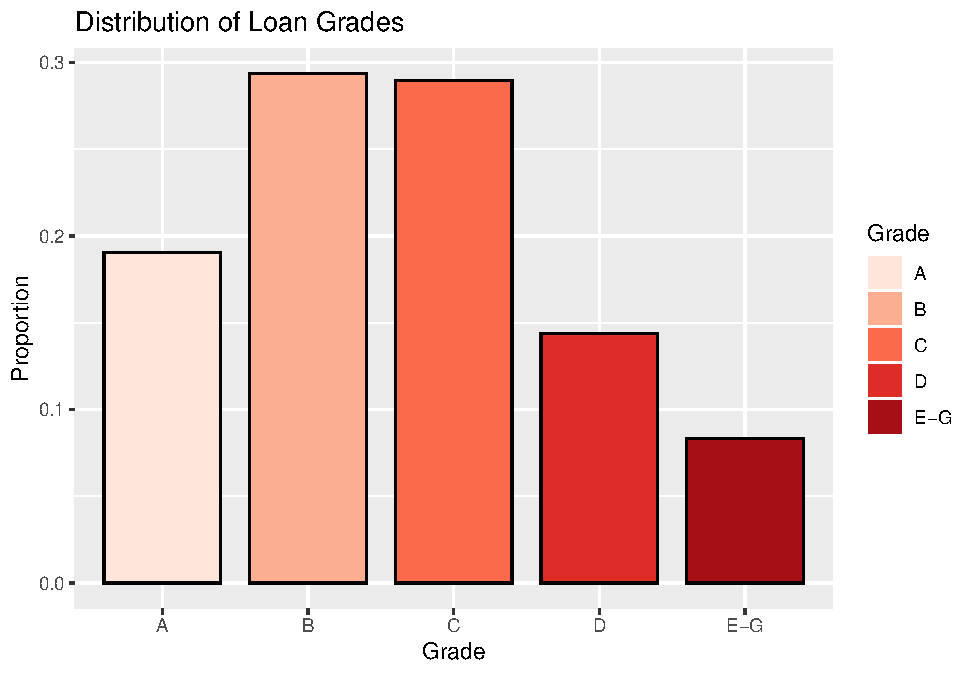
\includegraphics{An-Analysis-of-LendingClub-Loan-Grades_files/figure-latex/unnamed-chunk-1-1.pdf}

The conditional distribution of loan grades by application type isn't
too telling. The proportion of loan grades for individual applicants is
about the same as that for joint applicants.

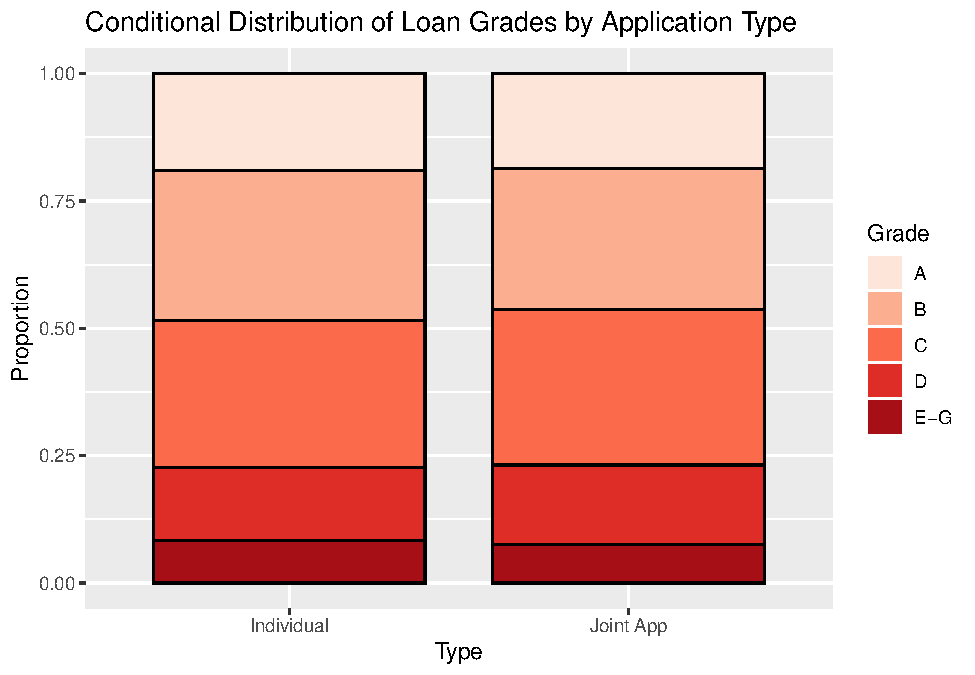
\includegraphics{An-Analysis-of-LendingClub-Loan-Grades_files/figure-latex/unnamed-chunk-2-1.pdf}

\begin{longtable}[]{@{}lrrrrr@{}}
\toprule
& A & B & C & D & E-G\tabularnewline
\midrule
\endhead
Individual & 0.1905676 & 0.2943460 & 0.2886296 & 0.1428907 &
0.0835661\tabularnewline
Joint App & 0.1854149 & 0.2782064 & 0.3046270 & 0.1562883 &
0.0754635\tabularnewline
\bottomrule
\end{longtable}

The conditional distribution of loan grades by home ownership reveals a
bit more about the data. Specifcally, we can see a noticeable difference
in the distribution of grades for the ``OTHER'' category compared to the
remaining home ownership categories.

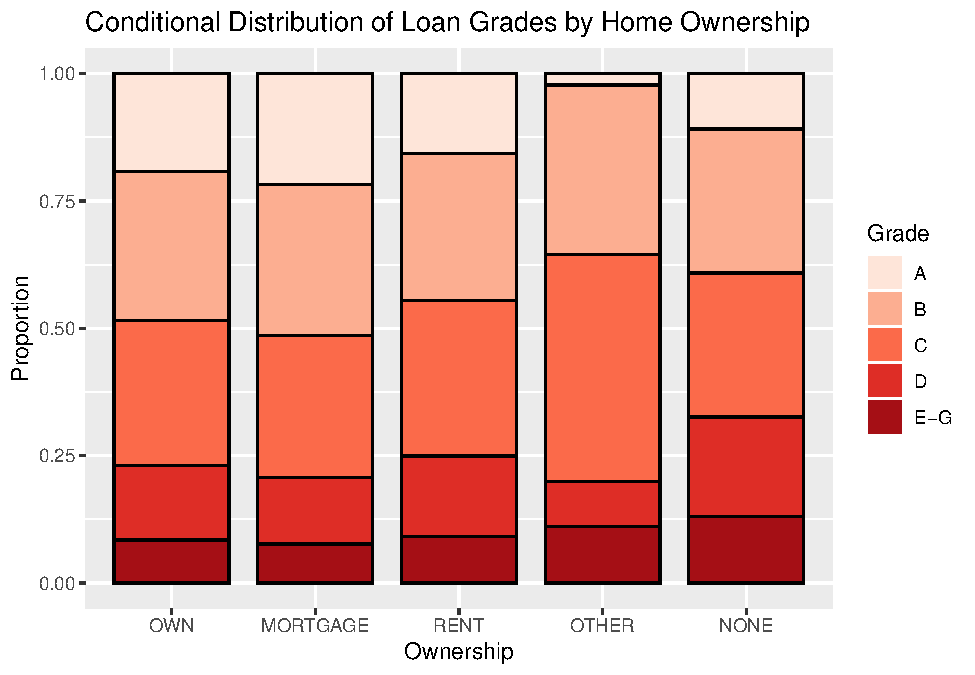
\includegraphics{An-Analysis-of-LendingClub-Loan-Grades_files/figure-latex/unnamed-chunk-3-1.pdf}

\begin{longtable}[]{@{}lrrrrr@{}}
\toprule
& A & B & C & D & E-G\tabularnewline
\midrule
\endhead
OWN & 0.1924881 & 0.2913036 & 0.2855623 & 0.1462761 &
0.0843699\tabularnewline
MORTGAGE & 0.2172712 & 0.2974222 & 0.2776133 & 0.1311165 &
0.0765768\tabularnewline
RENT & 0.1559376 & 0.2891622 & 0.3054611 & 0.1584755 &
0.0909636\tabularnewline
OTHER & 0.0222222 & 0.3333333 & 0.4444444 & 0.0888889 &
0.1111111\tabularnewline
NONE & 0.1086957 & 0.2826087 & 0.2826087 & 0.1956522 &
0.1304348\tabularnewline
\bottomrule
\end{longtable}

Looking at the mean loan amounts by grade, as the loans are graded as
riskier the means get larger.

\begin{longtable}[]{@{}lrrrrr@{}}
\toprule
& A & B & C & D & E-F\tabularnewline
\midrule
\endhead
Average Loan Amount (\$) & 14764.38 & 14235.71 & 15095.48 & 15783.47 &
18062.62\tabularnewline
\bottomrule
\end{longtable}

Breaking it up by loan grade, we can look at the density of the loans.
For grades A, B, and C, the distributions are right noticeably
right-skewed, with most of the loans be around \$10,000. For grades D
and E-G, the distributions of the amounts are still right skewed, but
not as pronounced. This shows that the riskier graded loans have a
greater spread of loan amounts, with a greater amount being closer to
\$40,000.

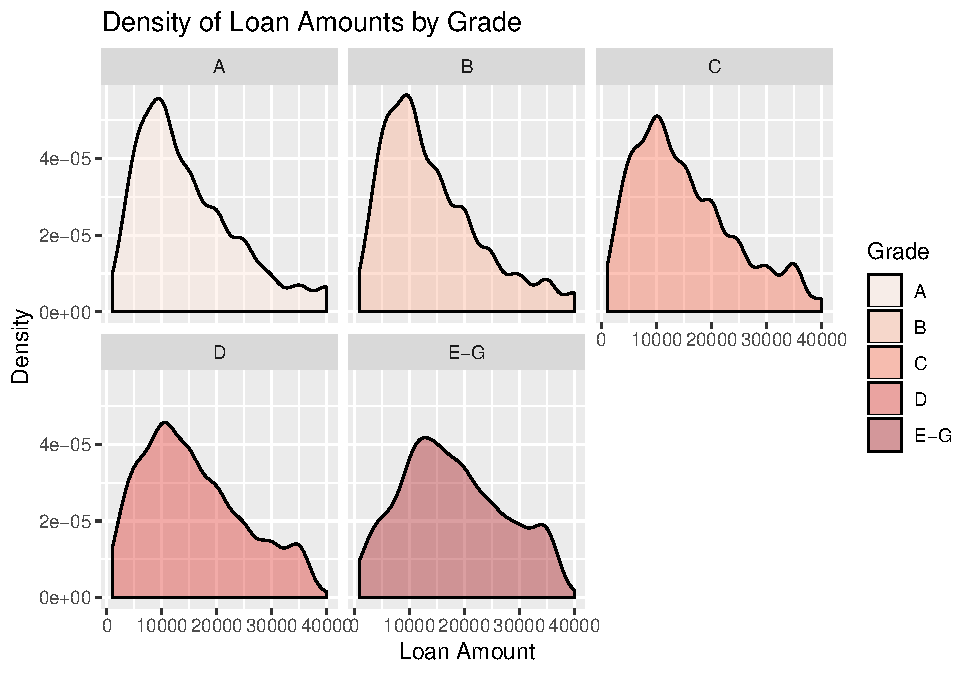
\includegraphics{An-Analysis-of-LendingClub-Loan-Grades_files/figure-latex/unnamed-chunk-5-1.pdf}

Looking at the densities divided by application type, the joint
applications have a wider spread of loan amounts, whereas the individual
applications are more right skewed.

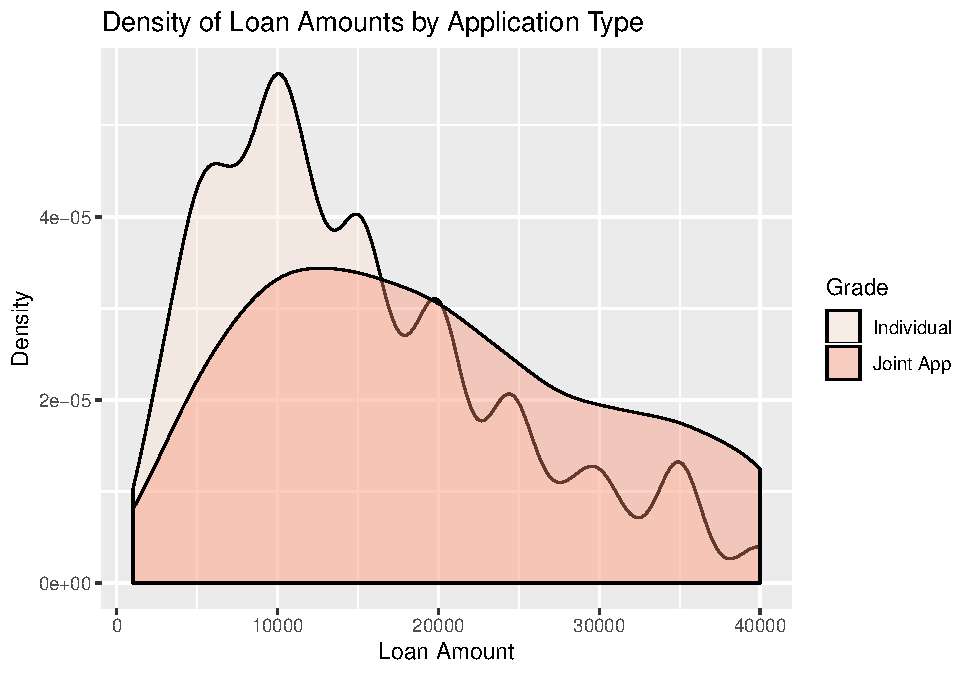
\includegraphics{An-Analysis-of-LendingClub-Loan-Grades_files/figure-latex/unnamed-chunk-6-1.pdf}

\hypertarget{model-selection}{%
\section{Model Selection}\label{model-selection}}

After looking at some summary statistics and visualizations, it's time
to use a multiple cumulative logistic regression model to predict loan
grades and understand which variables from our \emph{loans} data are
significant. The loan grades will be treated as ordinal. First, a model
with all of the predictor variables will be created to model the
cumulative probabilities for loan grades. Then alternative models with
less predictors will be compared to select the best model. After that,
we'll look at the significance of the different predictors and look at
their effects.

Below is the coefficient table for the model with Annual\_Income,
Application\_Type, Debt\_to\_Income, Home\_Ownership, Loan\_Amount, and
Mortgage Accounts. Every variable except some of the home ownership
dummy variables are significant in predicting the cumulative
probabilities.

\begin{longtable}[]{@{}lrrrr@{}}
\toprule
& Estimate & Std. Error & z value &
Pr(\textgreater{}\textbar{}z\textbar{})\tabularnewline
\midrule
\endhead
(Intercept):1 & -1.0954094 & 0.0468438 & -23.384298 &
0.0000000\tabularnewline
(Intercept):2 & 0.3703563 & 0.0458216 & 8.082577 &
0.0000000\tabularnewline
(Intercept):3 & 1.6771041 & 0.0474568 & 35.339566 &
0.0000000\tabularnewline
(Intercept):4 & 2.9176684 & 0.0519196 & 56.195928 &
0.0000000\tabularnewline
Annual\_Income & 0.0000047 & 0.0000003 & 15.363055 &
0.0000000\tabularnewline
Application\_TypeJoint App & 0.4024106 & 0.0601588 & 6.689135 &
0.0000000\tabularnewline
Debt\_to\_Income & -0.0189580 & 0.0013510 & -14.032687 &
0.0000000\tabularnewline
Home\_OwnershipOWN & -0.0341280 & 0.0429635 & -0.794348 &
0.4269929\tabularnewline
Home\_OwnershipRENT & -0.1677057 & 0.0315844 & -5.309763 &
0.0000001\tabularnewline
Loan\_Amount & -0.0000320 & 0.0000016 & -20.147413 &
0.0000000\tabularnewline
Mortgage\_Accounts & 0.0603496 & 0.0079395 & 7.601216 &
0.0000000\tabularnewline
\bottomrule
\end{longtable}

Below is the coefficient table with the Home\_Ownership variable
removed.

\begin{longtable}[]{@{}lrrrr@{}}
\toprule
& Estimate & Std. Error & z value &
Pr(\textgreater{}\textbar{}z\textbar{})\tabularnewline
\midrule
\endhead
(Intercept):1 & -1.0860229 & 0.0397771 & -27.302726 & 0\tabularnewline
(Intercept):2 & 0.3693499 & 0.0386034 & 9.567808 & 0\tabularnewline
(Intercept):3 & 1.7302129 & 0.0406366 & 42.577696 & 0\tabularnewline
(Intercept):4 & 2.9091518 & 0.0455828 & 63.821253 & 0\tabularnewline
Annual\_Income & 0.0000039 & 0.0000003 & 12.987711 & 0\tabularnewline
Application\_TypeJoint App & 0.3944882 & 0.0577645 & 6.829246 &
0\tabularnewline
Debt\_to\_Income & -0.0218640 & 0.0013547 & -16.139861 &
0\tabularnewline
Loan\_Amount & -0.0000316 & 0.0000016 & -19.991519 & 0\tabularnewline
Mortgage\_Accounts & 0.0889280 & 0.0071387 & 12.457243 &
0\tabularnewline
\bottomrule
\end{longtable}

Next, the AICs for the two models were compared and the model with
Home\_Ownership recieved a better score of 59,616.99, compared to
59,657.1 for the model without the Home\_Ownership variable.

The analysis of deviance output below doesn't show that any predictors
are not needed in the model.

\begin{longtable}[]{@{}lrrrrr@{}}
\toprule
& Df & Deviance & Resid. Df & Resid. Dev &
Pr(\textgreater{}Chi)\tabularnewline
\midrule
\endhead
Annual\_Income & 1 & 3.8654559 & 79990 & 60603.80 &
0.0492898\tabularnewline
Application\_Type & 1 & 0.6128146 & 79990 & 60600.54 &
0.4337300\tabularnewline
Debt\_to\_Income & 1 & 1.6806353 & 79990 & 60601.61 &
0.1948401\tabularnewline
Home\_Ownership & 2 & 1.4494287 & 79991 & 60601.38 &
0.4844629\tabularnewline
Loan\_Amount & 1 & 0.0004365 & 79990 & 60599.93 &
0.9833305\tabularnewline
Mortgage\_Accounts & 1 & 4.0499321 & 79990 & 60603.98 &
0.0441731\tabularnewline
\bottomrule
\end{longtable}

Below is the final model coefficient table for the cumulative
probabilities of the loan grades.

\begin{longtable}[]{@{}lrrrr@{}}
\toprule
& Estimate & Std. Error & z value &
Pr(\textgreater{}\textbar{}z\textbar{})\tabularnewline
\midrule
\endhead
(Intercept):1 & -1.0954094 & 0.0468438 & -23.384298 &
0.0000000\tabularnewline
(Intercept):2 & 0.3703563 & 0.0458216 & 8.082577 &
0.0000000\tabularnewline
(Intercept):3 & 1.6771041 & 0.0474568 & 35.339566 &
0.0000000\tabularnewline
(Intercept):4 & 2.9176684 & 0.0519196 & 56.195928 &
0.0000000\tabularnewline
Annual\_Income & 0.0000047 & 0.0000003 & 15.363055 &
0.0000000\tabularnewline
Application\_TypeJoint App & 0.4024106 & 0.0601588 & 6.689135 &
0.0000000\tabularnewline
Debt\_to\_Income & -0.0189580 & 0.0013510 & -14.032687 &
0.0000000\tabularnewline
Home\_OwnershipOWN & -0.0341280 & 0.0429635 & -0.794348 &
0.4269929\tabularnewline
Home\_OwnershipRENT & -0.1677057 & 0.0315844 & -5.309763 &
0.0000001\tabularnewline
Loan\_Amount & -0.0000320 & 0.0000016 & -20.147413 &
0.0000000\tabularnewline
Mortgage\_Accounts & 0.0603496 & 0.0079395 & 7.601216 &
0.0000000\tabularnewline
\bottomrule
\end{longtable}

\hypertarget{model-interpretation-and-visualiation}{%
\section{Model Interpretation and
Visualiation}\label{model-interpretation-and-visualiation}}

Now that we selected the best model, it's important to visualize the
effects of the variables on the probability of being given a certain
loan grade and to interpret the effects.

\textbf{\emph{Model Formula}}

A = 1, B = 2, C = 3, D = 4, E-G = 5

Below is the formula for the logit({[}Y\textless{}=J{]}) where J is some
number from 1-4, standing for the loan grades as shown above. \(J_1\),
\(J_2\), \(J_3\), and \(J_4\) are binary and depend upon J.

\[logit({[Y<=J]}) = -0.6868569(J_1) + 0.7285327(J_2) +2.0833608(J_3) + 3.2860989(J_4) +\\ + 0.0000024(AnnualIncome) -0.0287011(DebtToIncome)\\ - 0.0000285(LoanAmount) + 0.0549374(MortgageAccounts) + 0.32860989I(JointApp)\\ - 0.0287011I(MORTGAGE) - 0.0245795I(OWN) - 0.271375I(RENT)\]

Below is the formula for the odds of being Y\textless{}=J.

\[odds({[Y<=J]}) = e^{-0.6868569(J_1) + 0.7285327(J_2) + 2.0833608(J_3) + 3.2860989(J_4)} *\\ e^{0.0000024(AnnualIncome) - 0.0287011(DebtToIncome)} *\\ e^{- 0.0000285(LoanAmount) + 0.0549374(MortgageAccounts) + 0.32860989I(JointApp)} *\\ e^{- 0.0287011I(MORTGAGE) - 0.0245795I(OWN) - 0.271375I(RENT)}\]

\textbf{\emph{Interpretations}}

Below are formal interpretations of two of the variables used in the
model.

Debt\_to\_Income effects:

``For a 1 unit increase in the debt-to-income ratio, the odds of falling
at or below a grade X decrease by 3\%''

Application\_Type effects:

``If an application is joint, then the odds of falling at or below grade
X increases by 38.9\% from that of the individual application
baseline.''

\textbf{\emph{Model Visualizations}}

Below are four graphs. For the first two, they visualize the cumulative
probabilities of loan grades as the debt to income ratio increases for
individual applications and joint applications. For both of these
graphs, the home ownership is held constant at ``MORTGAGE'', the number
of mortgage accounts held constant at the mean 1.56, loan amount at the
mean \$15,125.61, and income held constant at the mean \$78,257.95.

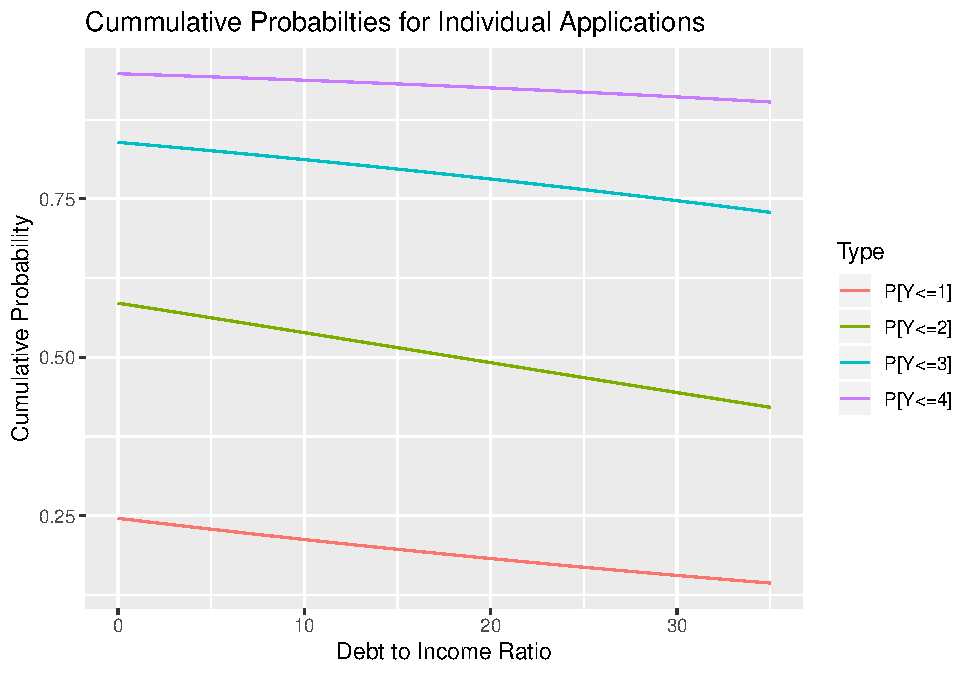
\includegraphics{An-Analysis-of-LendingClub-Loan-Grades_files/figure-latex/unnamed-chunk-12-1.pdf}
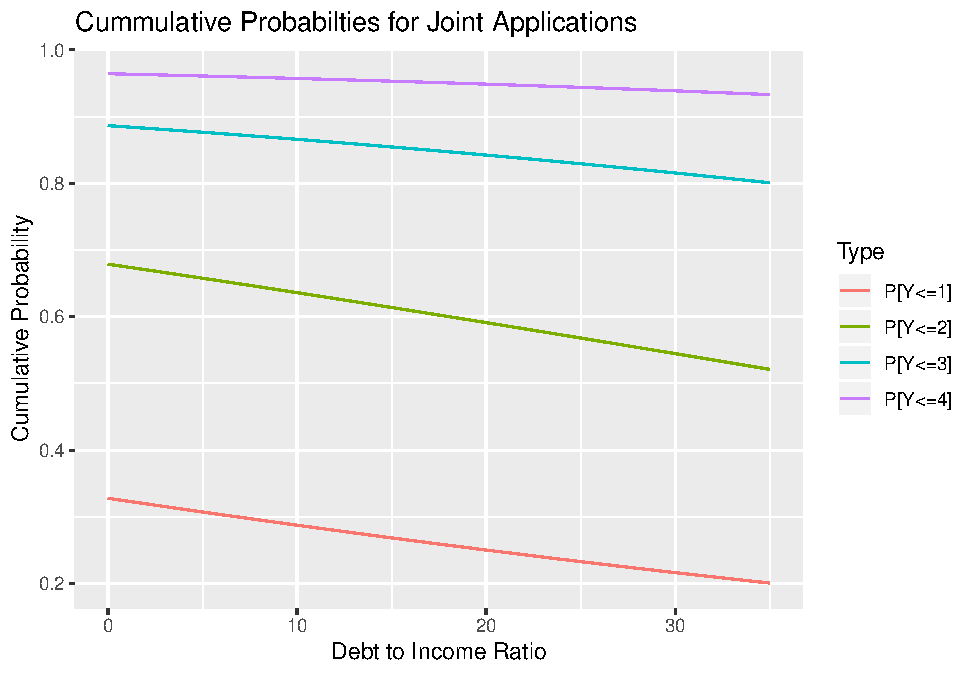
\includegraphics{An-Analysis-of-LendingClub-Loan-Grades_files/figure-latex/unnamed-chunk-12-2.pdf}

The last two visualize the probabilities of a loan receiving different
grades for joint and individual applicants as the debt to income ratio
increases. Again, for both of these graphs, the home ownership is held
constant at ``MORTGAGE'', the number of mortgage accounts held constant
at the mean 1.56, loan amount at the mean \$15,125.61, and income held
constant at the mean \$78,257.95.

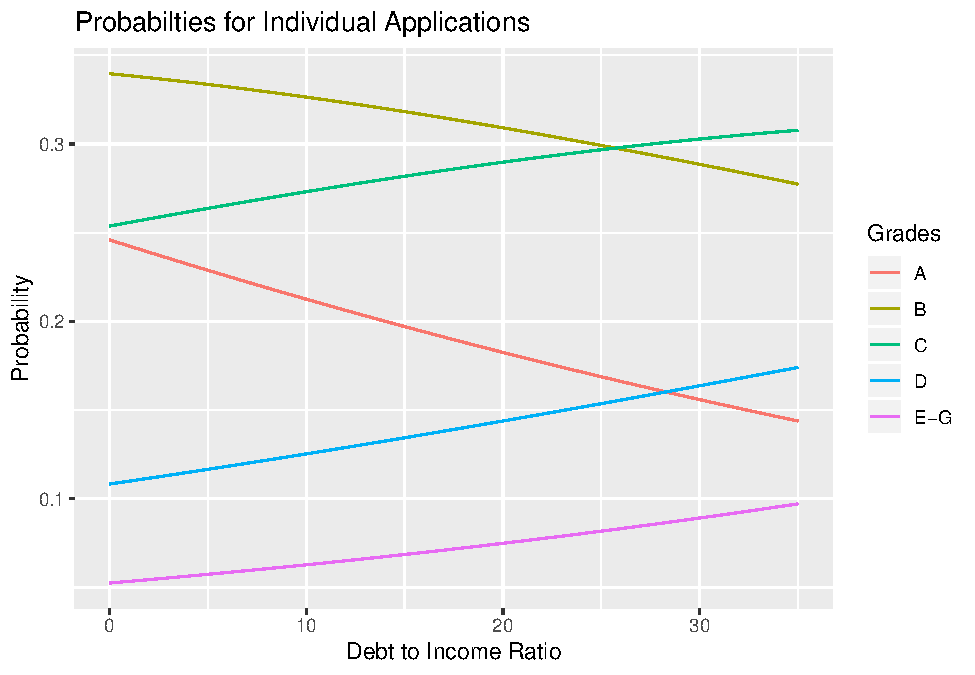
\includegraphics{An-Analysis-of-LendingClub-Loan-Grades_files/figure-latex/unnamed-chunk-13-1.pdf}
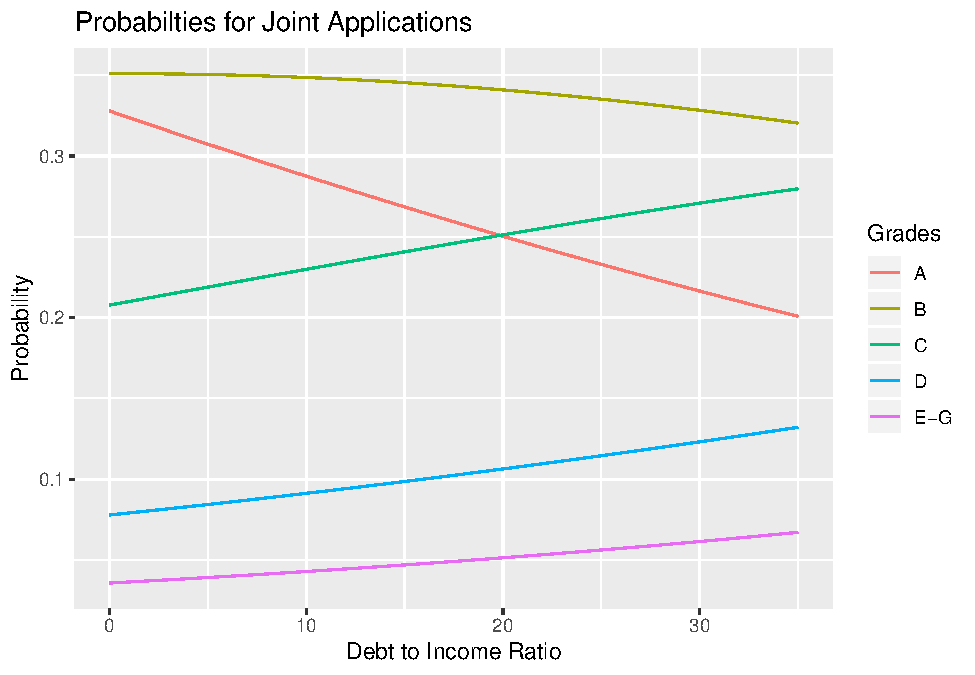
\includegraphics{An-Analysis-of-LendingClub-Loan-Grades_files/figure-latex/unnamed-chunk-13-2.pdf}





\newpage
\singlespacing 
\end{document}
